\section{Analisi dei dati}\label{sec:analisi}
\normalsize
In questa sezione saranno analizzati i dati di SkillCraftI per cercare di capire la struttura dei dati e correggere eventuali problemi che il dataset potrebbe avere. Per fare questo saranno usate le librerie Python Matplotlib e Seaborn, che permettono di graficare i dati per renderli più leggibili e interpretabili.   
\subsection{Bilanciamento del dataset}\label{ssec:bilanciamento}
\normalsize
I rank di starcraft sono per loro natura sbilanciati, dal sito Liquipedia, un’enciclopedia online a tema videogiochi, si può leggere come sono strutturare le leghe del gioco e gli obbiettivi che si sono posti gli sviluppatori quando le hanno create. \\*\\*
La distribuzione a cui puntavano gli sviluppatori è come segue:
\begin{itemize}
	\item Grand Master 1000 giocatori
	\item Master 2\%
	\item Diamante 18\%
	\item Platino 20\%
	\item Oro 20\%
	\item Argento 20\% 
	\item Bronzo 20\%
\end{itemize}

Nella realtà le cifre sono destinate ad essere leggermente diverse, ma la proporzione è corretta a grandi linee, in più oltre a questi rank nel data set possiamo trovare anche i giocatori professionisti. Questa ulteriore divisione è stata aggiunta perché, anche se i grand master possono essere considerati un elite tra i giocatori, il divario le loro capacità e quelle dei professionisti è considerevole. \\*
\begin{center}
	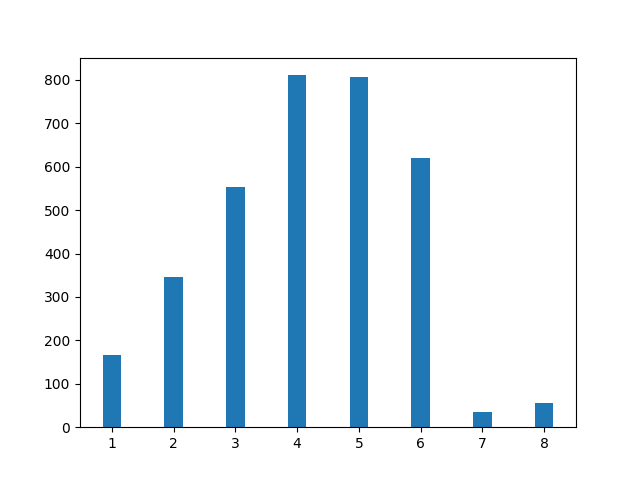
\includegraphics[scale=0.9]{../figures/sbilanciamento.PNG}
\end{center}
\par
Come previsto il dataset è sbilanciato, questo comporta che bisognerà prestare attenzione a come vengono raggruppati i sample durante l’addestramento dei modelli. Oltre a questo, l’unica altra anomalia che è possibile individuare è che al contrario delle aspettative ci sono più professionisti che Grand Master, questo non è rispecchiato nella realtà ed è dovuto al modo in cui sono stati campionati i dati, ma ai fini della classificazione non dovrebbe creare grossi problemi.

\subsection{Elementi nulli}\label{ssec:nulli}
\normalsize
Per la buona riuscita dell’addestramento è necessario rimuovere gli elementi nulli e il nostro dataset ne ha alcuni, ora cercheremo di capire quanti sono e come sono distribuiti per trovare una soluzione al problema.\\*\\*
Il grafico sotto rappresenta il numero totale dei valori nulli per ogni rank divisi per la feature a cui appartengono.
\begin{center}
	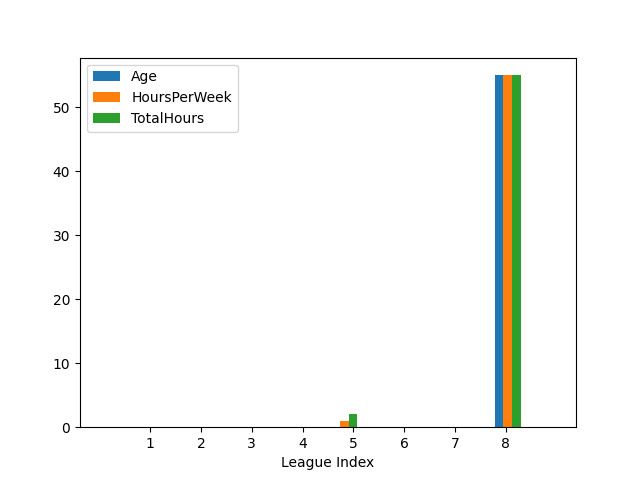
\includegraphics[scale=0.9]{../figures/Nan_distribuzione.PNG}
\end{center}